\documentclass{modernsimplecv}
% try out different fonts: classic, fira, raleway, chivo
\usepackage[utf8]{inputenc}
\usepackage[margin=1cm, a4paper]{geometry}

% ------------------------------------------------------------------------------------
% you can try out different fonts here by commenting the following lines in and out
% -----------------------------------------------------------------------------------
\usepackage[default]{raleway}
%\usepackage[sfdefault]{FiraSans} %% option 'sfdefault' activates Fira Sans as the default text font\renewcommand*\oldstylenums[1]{{\firaoldstyle #1}}\normalfont
%\usepackage[familydefault,light]{Chivo} 
%\usepackage[sfdefault,light,condensed]{roboto}
%\usepackage[default]{cantarell}
%\usepackage[sfdefault]{AlegreyaSans}


\usepackage{beuron}
\usepackage{LobsterTwo}%if not suposed to be main font, load other main font after this



%------------------------------------------------------------------ Variablen

\newlength{\rightcolwidth}
\newlength{\leftcolwidth}
\setlength{\leftcolwidth}{0.48\textwidth}
\setlength{\rightcolwidth}{0.47\textwidth}

%------------------------------------------------------------------
\title{modern-simple-CV}
\author{\LaTeX{} Ninja}
\date{August 2019}

\pagestyle{empty}
\begin{document}


\thispagestyle{empty}
%-------------------------------------------------------------



\tikz[remember picture,overlay] {%
\node[rectangle, fill=white, anchor=north, minimum width=\paperwidth, minimum height=5cm](header) at (current page.north){};%
}

\begin{minipage}[t]{0.21\textwidth}
\vspace{0pt} % Trick for alignment
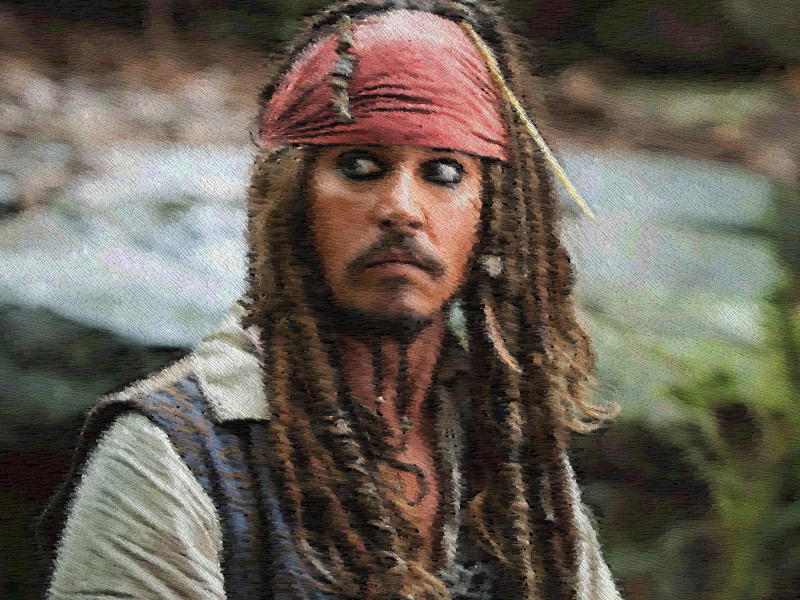
\includegraphics[width=\textwidth]{jack.jpg}\hspace{1em}
\end{minipage}
\hfill
\begin{minipage}[t]{0.77\textwidth}
\vspace{0pt} % Trick for alignment
\begin{shaded*}

\begin{minipage}[t]{0.4\textwidth}
\vspace{0pt} % Trick for alignment
% here the fancy font can be taken out by removing \LobsterTwo
{\par\centering\huge\LobsterTwo{Jack Sparrow}} \\[0.3cm]
\faGlobe~ Nationality: english\\
\faBirthdayCake~ 1690 \\
\faMapMarker~ on a ship \\

{\small
\faGraduationCap~ \underline{Titles:} Dr. Dr. Captain \\
\faCommentsO~ \underline{Languages:} \emph{English} C2, \emph{French} B2.}
\end{minipage}\hfill
\begin{minipage}[t]{0.55\textwidth}
\vspace{0pt} % Trick for alignment
\faPhone~ 0999/999 6767400 \\
\faAt~ \protect\url{jack@sparrow.com} \\

\faEnvelopeO~ The Black Pearl \\ 
\faMapMarker~ Tortuga \\

%\aiAcademiaSquare 
\faFont~ \protect\url{https://academia.edu/JackSparrow} \\
\faGithub~ \protect\url{github.com/sparrow} \\
%\aiOrcid 
\faCircle~ \protect\url{orcid.org/0000-0000-0000-0000} \\
\end{minipage}
\hfill
\end{shaded*}
\end{minipage}\\[15pt]


%------------------------------------------------

% hier muss die "unsichtbare" Überschrift rein, weil er sonst nicht die Paracols startet... komisch...
\subsection*{}
\vspace{-3em}

\setlength{\columnsep}{1.5cm}
\columnratio{0.48}[0.47]
\begin{paracol}{2}
\hbadness5000
%\backgroundcolor{c[1]}[rgb]{1,1,0.8} % cream yellow for column-1 %\backgroundcolor{g}[rgb]{0.8,1,1} % \backgroundcolor{l}[rgb]{0,0,0.7} % dark blue for left margin

\paracolbackgroundoptions

% 0.9,0.9,0.9 -- 0.8,0.8,0.8


\footnotesize
{

\small
\section*{Short Resumé}

\begin{minipage}[t]{\leftcolwidth}
\begin{tabular}{r| p{0.6\textwidth} c}
    \cvevent{2018--2021}{Captain of the Black Pearl}{Lead}{East Indies}{Finally got the goddamn ship back. \lorem}{disney.png} \\
    \cvevent{2019}{Freelance Pirate}{Bucaneering}{Tortuga}{This and that. The usual, aye?}{medal.jpeg} \\
    \cvevent{2016--2017}{Captain of the Black Pearl}{Lead}{Tortuga}{Found a secret treasure, lost the ship.}{medal.jpeg}
\end{tabular}

\vspace{4em}

\small
\section*{Lots of Information}

\begin{tabular}{r| p{0.6\textwidth} c}
    \cvevent{2018--2021}{Captain of the Black Pearl}{Lead}{East Indies}{Finally got the goddamn ship back.}{disney.png} \\
    \cvevent{2019}{Freelance Pirate}{Bucaneering}{Tortuga}{This and that. The usual, aye? \lorem}{medal.jpeg} \\
    \cvevent{2016--2017}{Captain of the Black Pearl}{Lead}{Tortuga}{Found a secret treasure, lost the ship.}{medal.jpeg}
\end{tabular}

\vspace{4em}
\end{minipage}

\begin{minipage}[t]{\leftcolwidth}
\section*{Degrees}
\begin{tabular}{r p{0.6\textwidth} c}
    \cvdegree{1710}{Captain}{Certified}{Tortuga Uni}{}{disney.png} \\
    \cvdegree{1715}{Bucaneering}{M.A.}{London}{}{medal.jpeg} \\
    \cvdegree{1720}{Bucaneering}{B.A.}{London}{}{medal.jpeg}
\end{tabular}
\end{minipage}\hfill

\vspace{3em}

\begin{minipage}[t]{\leftcolwidth}
\section*{Certificates \& Grants}
\begin{tabular}{>{\footnotesize\bfseries}r >{\footnotesize}p{0.55\textwidth}}
    1708 & Captain's Certificates \\
    1710 & Travel grant \\
    1715--1716 & Grant from the Pirate's Company\\
    1708 & Captain's Certificates \\
    1710 & Travel grant \\
    1715--1716 & Grant from the Pirate's Company
\end{tabular}
\bigskip

\end{minipage}\hfill


\vspace{2em}

\begin{minipage}[t]{\leftcolwidth}
\section*{Lots of Information}
\begin{tabular}{r| p{0.6\textwidth} c}
    \cvevent{2018--2021}{Captain of the Black Pearl}{Lead}{East Indies}{Finally got the goddamn ship back. \lorem}{disney.png} \\
    \cvevent{2019}{Freelance Pirate}{Bucaneering}{Tortuga}{This and that. The usual, aye?}{medal.jpeg} \\
    \cvevent{2016--2017}{Captain of the Black Pearl}{Lead}{Tortuga}{Found a secret treasure, lost the ship.}{medal.jpeg}
\end{tabular}

\vspace{4em}

\small
\section*{Lots of Information}

\begin{tabular}{r| p{0.6\textwidth} c}
    \cvevent{2018--2021}{Captain of the Black Pearl}{Lead}{East Indies}{Finally got the goddamn ship back.}{disney.png} \\
    \cvevent{2019}{Freelance Pirate}{Bucaneering}{Tortuga}{This and that. The usual, aye? \lorem}{medal.jpeg} \\
    \cvevent{2016--2017}{Captain of the Black Pearl}{Lead}{Tortuga}{Found a secret treasure, lost the ship.}{medal.jpeg}
\end{tabular}

\vspace{4em}
\end{minipage}

}
%-----------------------------------------------------------
\switchcolumn

\begin{minipage}[t]{\rightcolwidth}
\section*{Short Resumé}

\begin{tabular}{r| p{0.6\textwidth} c}
    \cvevent{2018--2021}{Captain of the Black Pearl}{Lead}{East Indies}{Finally got the goddamn ship back.}{disney.png} \\
    \cvevent{2019}{Freelance Pirate}{Bucaneering}{Tortuga}{This and that. The usual, aye?}{medal.jpeg} \\
    \cvevent{2016--2017}{Captain of the Black Pearl}{Lead}{Tortuga}{Found a secret treasure, lost the ship.}{medal.jpeg}
\end{tabular}

\end{minipage}

\vspace{2em}

\lineheading{\rightcolwidth}{Code}{\faCode}{black}

\lipsum[10]



\bigskip

\section{Programming} 
{\small
\lipsum[20]

}
\bigskip

\begin{skillsection}{\rightcolwidth}
    \cvitem{\faStar\faStar\faStar\faStar\faStar}{Python: Machine Learning, \dots}
    \cvitem{\faStarO\faStar\faStar\faStar\faStar}{Bootstrap}
            \cvitem{\faStarO\faStarO\faStar\faStar\faStar}{jQuery}
        \cvitem{\faStarO\faStarO\faStarO\faStar\faStar}{Databases}
    \cvitem{\faStarO\faStarO\faStarO\faStarO\faStar}{c++}
\end{skillsection}


\bigskip



\vspace{4em}


\begin{minipage}[t]{\rightcolwidth}
\section*{Publications}
\begin{tabular}{>{\footnotesize\bfseries}r >{\footnotesize}p{0.7\textwidth}}
    1729 & \emph{How I almost got killed by Lady Swan}, Tortuga Printing Press. \\
    1720 & ``Privateering for Beginners'', in: \emph{The Pragmatic Pirate} (1/1720).\\
    1729 & \emph{How I almost got killed by Lady Swan}, Tortuga Printing Press. \\
    1720 & ``Privateering for Beginners'', in: \emph{The Pragmatic Pirate} (1/1720).\\
    1729 & \emph{How I almost got killed by Lady Swan}, Tortuga Printing Press. \\
    1720 & ``Privateering for Beginners'', in: \emph{The Pragmatic Pirate} (1/1720).
\end{tabular}
\bigskip

\section*{Talks}
\begin{tabular}{>{\footnotesize\bfseries}r >{\footnotesize}p{0.6\textwidth}}
    Nov. 1726 & ``How I lost my ship (\& and how to get it back)'', at: \emph{Annual Pirate's Conference} in Tortuga, Nov. 1726. \\
    Nov. 1726 & ``How I lost my ship (\& and how to get it back)'', at: \emph{Annual Pirate's Conference} in Tortuga, Nov. 1726. \\
    Nov. 1726 & ``How I lost my ship (\& and how to get it back)'', at: \emph{Annual Pirate's Conference} in Tortuga, Nov. 1726.
\end{tabular}
\end{minipage}









\end{paracol}

\vfill{} % Whitespace before final footer

%----------------------------------------------------------------------------------------
%	FINAL FOOTER
%----------------------------------------------------------------------------------------
\setlength{\parindent}{0pt}
\begin{minipage}[t]{\textwidth}
\begin{center}\fontfamily{\sfdefault}\selectfont \color{black!70}
{\small Jack Sparrow \icon{\faEnvelopeO}{black}{} The Black Pearl \icon{\faMapMarker}{black}{} Tortuga \icon{\faPhone}{black}{} 0099/333 5647380 
\icon{\faAt}{black}{} \protect\url{jack@sparrow.com}
}
\end{center}
\end{minipage}

\end{document}
